\section{Introduction}
\noindent
\textbf{Localization} is the problem related to the \textbf{estimation} of the position of a \textbf{target}. Other problems are those related to the \textbf{detection} (whether a target is present or not) and \textbf{tracking} that is we track the position of a \textbf{moving target}.\\
Nowadays the focus is in particular on \textbf{Indoor Localization} whose mathematical modeling is quite challenging due to the presence of \textit{multipath} and \textit{reflecting surfaces}. For these reasons there is not an available \textbf{unified approach}. \\
GPS is not usable for indoor localization, the so called \textbf{WSN (Wirelless Sensor Networks)} are used for this purpose. A WSN is essentially a network of devices equipped  with sensors. We can find two main approaches: 
\begin{enumerate}
    \item \textbf{Triangulation and Trilateration}: in this case we assume that the target is a \textbf{transmitting device} that broadcasts a signal. The former method deploy the \textbf{direction of arrival} of such signal, the latter use instead the \textbf{distance} from the source's signal (\textit{id est} the target). For this approach, in the case that the measurement are exact, 3 non-aligned sensors are sufficient, alternatively the higher number of sensors, the higher precision reached.
    \item \textbf{Fingerprinting methods} refers to techniques that match the \textbf{fingerprint} of some characteristics of a signal which is \textbf{location-dependent}. For our purposes we consider the \textbf{Received Signal Strength} or \textbf{RSS}.
\end{enumerate}

\section{RSS-fingerprinting: general description }
In general for all \textbf{Fingerprinting method}, we identify \textbf{two phases}:
\begin{enumerate}
    \item \textbf{Training phase} in which we collect the fingerprints of a scene; 
    \item \textbf{Runtime phase} in which we match the online measurement with the closest a-priori location fingerprints.
\end{enumerate}
As we said, we focus our attention on \textit{RSS-fingerprinting}.

\subsection{(Phase 0) Initialization }
Given the room where the localization has to be done, we deploy the WSN in some way (For example: grid deployment, or random (uniform) deployment, split the room into $p$ cells.   \textbf{Localize the target} $\longrightarrow$ detect in which cell the target is placed.

\begin{figure}[h]
    \centering
    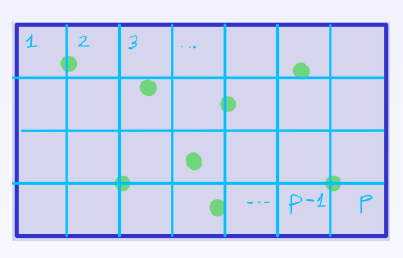
\includegraphics{images/RSS-cells.png}
    \caption{(Phase 0) - Initialization}
    \label{fig:RSS-Cells}
\end{figure}

\subsection{(Phase 1) Training phase}
We put the target in each cell. According to the fact that the target itself broadcasts a signal, \textbf{each sensor} measures and stores the RSS, and create a \textbf{signature map} or \textbf{dictionary}. More specifically, the dictionary can be represented by a matrix $D$, in which each entry $D_{i,j} $ denotes the RSS-measurement the sensor $i$ takes when the target is in the $j$-th cell. \\
\textbf{Each sensor} builds its own dictionary, and the WSN builds an \textbf{overall dictionary} $D\in \mathbb{R}^{q,p}$.\\
This phase takes some time and requires that the nodes of the network saved the information, it makes the runtime phase more accurate. 

\begin{figure}[h]
    \centering
    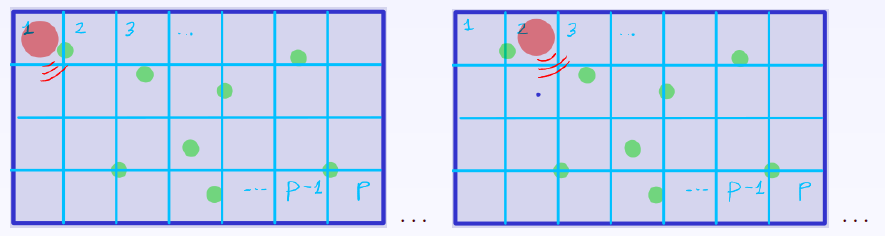
\includegraphics[scale=0.8]{images/RSS-training.png}
    \caption{(Phase 1) - Training phase}
    \label{fig:enter-label}
\end{figure}

\subsection{(Phase 2): Runtime phase}
Is the phase in which the localization is performed. Each sensor takes a measurement $y_i$, the $j$-th column of the dictionary indicates the $j$-th cell of the room in which the target is located!  

\begin{figure}[h]
    \centering
    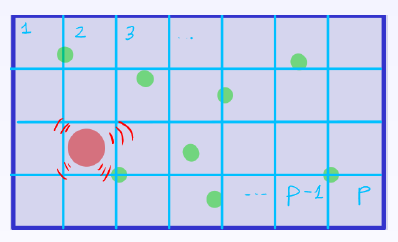
\includegraphics{images/RSS-Runtime.png}
    \caption{(Phase 2) - Runtime phase}
    \label{fig:enter-label}
\end{figure}

\noindent
If there is one target, then one of the columns of the dictionary would correspond to the measurement (in theory), then the target is located in the $j$-th cell where $j$ is such that $y=D_j$, with $D_j$ the $j-th$ column of the dictionary but usually, we can have \textit{multiple target} in the same room moreover it's very difficult that $y=D_j$ due to the presence of noise on sensors.\\

Then, in this scenario we have that the vector of measurements $y$ is a sum of a subset of the columns of the matrix $D$, to which we must add an additional term related to the noise. We have: 
\begin{equation} \label{eq: prob_loc}
	y=Dx+\text{noise}
\end{equation}
Where $x\in\{0,1\}^p$ and $x_i=1$ when in the i-th cell there is a target. \\
A further observation which can be done is that, in the real problems of \textit{indoor localization} the number of the targets one would like to localize is \textbf{much smaller} than the number of the cells, this leads to the sparsity of the solution $x\in\mathbb\{0,1\}^p$. 
Summarizing: (i) We want to find a solution to the problem (\ref{eq: prob_loc}), (ii) We know that such solution is \textbf{sparse}. Then,
\begin{equation}
	x^*=\text{arg}\min_{x\in\{0,1\}^p} \frac{1}{2} \lVert y-Dx \rVert_2^2 + \lambda \lVert x \rVert_1
 \end{equation}
This type of formulation leads to a \textbf{mixed integer} combinatorial problem, that again is NP-hard, so non-tractable. We can relax the constraint $x\in\{0,1\}^p$ into $x\in\mathbb{R}^p$, obtaining:
\begin{equation} \label{eq: loc_LASSO}
	x^*=\text{arg}\min_{x\in\mathbb{R}^p} \frac{1}{2} \lVert y-Dx \rVert_2^2 + \lambda \lVert x \rVert_1
\end{equation}
This is the problem of LASSO in the original formulation. {\color{red} It is important to remember that: } the solution of the problem (\ref{eq: loc_LASSO}) is not the original $x$ due to: (i) the presence of the noise, (ii) a bias introduced by the $\ell_1$-regularization term which in part promotes sparsity on the other hand inserts an error. One can use of course the \textbf{IST Algorithm} to find a solution.

\section{Localization under sparse sensor attacks}
\noindent
Assume that, in a realistic way, the training phase is \textit{attack-free}, therefore the matrix $D$ is attack free. Let us focus the attention again in the runtime phase.\\
What if the sensors were under adversarial attacks? One can apply the theory we developed in the former chapter! Then, we assume that the sensors under attacks are much smaller than the total number $q$ of them. In this context the equation (\ref{eq: prob_loc}) becomes: 
\begin{equation}
	y=Dx+a+noise	
\end{equation}
Then, the formulation of problem changes as follows:\\


\hspace*{-5mm}
\begin{tikzpicture}
	\node [mybox] (box){%
		\begin{minipage}{.96\textwidth}     %Larghezza del box
			\begin{equation}
				x^*=\text{arg}\min_{x\in\mathbb{R}^p} \frac{1}{2} \lVert y-Dx-a \rVert_2^2 + 
				\lambda_1 \lVert x \rVert_1+
				\lambda_2\lVert a \rVert_1
			\end{equation}
		\end{minipage}
	};
\end{tikzpicture}


where we are using different weights $\lambda_1, \lambda_2$ to give more or less importance to the term related to the solution $x$ and to the attack $a$. According to this novel aspect, the risen problem is a \textbf{weighted LASSO}. \textbf{IST algorithm} continues to work, as we saw in the case of presence of \textit{non-sparse} part of the solution in the case of SSE under adversarial attacks.

\noindent
\section{Other approaches to Localization}
The approach we have just seen is not the only one. Next paragraphs are in order to give some alternatives which differ from the first we have presented in computational complexity, time of convergence and so on.

\subsection{k-Nearest Neighbour (K-NN)}
Assume to know that there is only \textbf{one target}, given the vector $y\in \mathbb{R}^q$, we could find the $j-th$ column of the dictionary $D$ that is the \textbf{nearest} with respect to $y$. The localization problem in this specific scenario becomes: 
\begin{equation} \label{eq:knn_1}
	\hat{j} = \text{arg}\min_{j=1,...,p} \lVert D_j-y \rVert_2^2
\end{equation}
where $D_j$  is the $j$-th column of $D$. Note that in the problem there is not the factor $\frac{1}{2}$ but from the moment we have a minimization problem nothing changes.\\
RSS is additive so we can localize more than one target in the \textit{runtime phase}. Suppose that the targets are $k=2$, the vector $y$ can be seen as a sum of the columns, so the problem (\ref{eq:knn_1}) gets transformed in:
\begin{equation}
	(\hat{j_1}, \hat{j_2}) = \text{arg}\min_{(j_1, j_2)=1,...,p} 
	\lVert D_{j_1}+D_{j_2}-y \rVert_2^2
\end{equation} 

In general, we have to check a number of configurations that is equal to $\binom{p}{k} \rightarrow$ \textbf{NP-Hard}. Note that: this approach can be used if we have small $p, k$ otherwise other techniques ought to be used in order to promote efficiency.

\subsection{Linear Regression (noise-free case)}
If we have multiple targets, in absence of noise the localization problem could be formulated as a \textbf{binary linear regression}. We have to solve in $x$ the equation $y=Dx$ and add the constraints about the $x$ domain and sparsity. Then, it is obtained:
\begin{equation}
	\begin{aligned}
		Dx&=y\\
		&\text{s.t.} \ x\in\{0,1\}^p, \ \sum_{j=1}^{p}x_j=k
	\end{aligned}
\end{equation}
Even in this case it has been risen a mixed-integer combinatorial problem $\rightarrow$ NP-Hard. The choice should be taken in an accurate way according to the dimension of the problem.

\section{Some comments on the setting}
These algorithms assume that there is a \textbf{Fusion Center} where data from the sensors are collected. In this way: the Fusion Center stores the whole dictionary $D$ and the runtime measurements, so that it can run the localization algorithm which is nothing but one of the exposed methods.
